\subsubsection*{Preliminares}
La capa de Enlace (Data Link) se subdivide en dos capas, la primera \texttt{LLC} (Logical Link Control) que interactúa con la capa superior, y la de abajo es la \texttt{MAC} (Media Access Control) que interactúa con la capa física de abajo. Antes de enviar los datos, hay un tiempo de inactividad antes de que comience la transmisión, esto para que cada uno de los nodos se estabilice despues de la trama anterior.

\subsection*{Preambulo}
Un nodo comienza la transmisión enviando una secuencia  de preambulo de 7 \texttt{Bytes}, seguidos de un \texttt{Byte} llamado \texttt{SFD} (Start of Frame Delimiter). Esto consiste en una secuencia de 7 octetos con \texttt{1}s y \texttt{0}s intercalados (\texttt{10101010}) y seguido a estos, el \texttt{SFD} (\texttt{10101011}) que indica que el preambulo terminó y ya comienza el frame. El propósito del preambulo es dar tiempo al receptor en cada nodo para lograr sincronizar el reloj de datos de recepción con el de transmisión. Un concepto necesario para entender esto a mas profundidad es el Self-Clocking Signal\footnote{ En Telecomunicaciones y electrónica, una señal de este tipo es una que puede decodificarse sin la necesidad de una señal de reloj separada u otra fuente de sincronización, Esto generalemente se realiza mediante la inclusión de información de sincronización integrada dentro de la señal.}.

\subsection*{Codificación Manchester}
Es un método de condificación eléctrica de una señal binaria en el que en cada tiempo de bit hay una transición entre dos niveles de señal. Es autosíncrona, ya que en cada bit se puede obtener la señal de reloj lo que hace precisa una sincronización del flujo de datos. Una desventaja seria que requiere el doble de ancho de banda que una transmisión asíncrona. \\ ${ }$ \\
Las señales de datos y de reloj se combinan en una sola que autosincroniza el flujo de datos. Cada bit codificado contiene una transición en la mitad del intervalo de duración de los bits, de negativo a positivo representa un \texttt{1} y de positivo a negativo un \texttt{0}.
\subsubsection*{Codificación Manchester Diferencial}
Es una variacion del anterior , un bit \texttt{1} se indica por la ausencia de transición al inicio del intervalo y un bit \texttt{0} se indica por la presencia de una transición al inicio existiendo una transición en el centro del intervalo.
\\ ${ }$\\
Este es el esquema de codificación Manchester: \\
\pagebreak
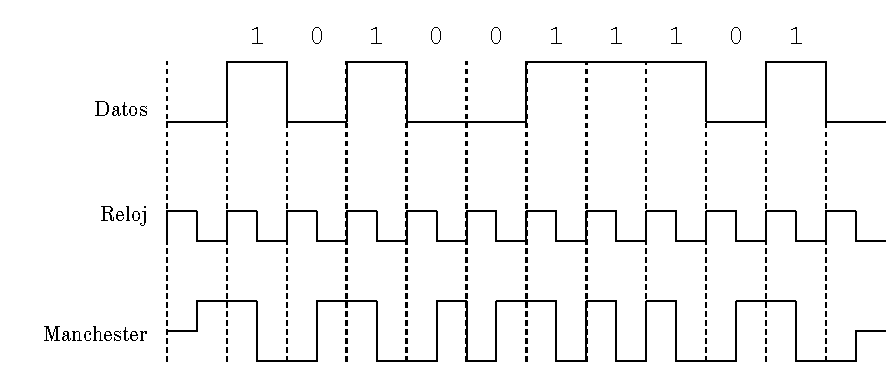
\includegraphics[page=1,scale=0.9]{Manchester.pdf}


%\begin{figure}[ht!]
%\centering
%\scalebox{.5}{
%\import{images/}{HDLCim.pdf_tex}
%}
%\caption{Ejemplo de la Trama.}
%\end{figure}
